% =============================================================================
% PSI512 - Topicos em Computacao em Nuvem (2026) - Trabalho Avaliativo 1
% Artigo tecnico - modelo SBC (coluna unica)
%
% COMO TRABALHAR NESTE ARQUIVO
%
% Cada secao tem um comentario dizendo QUEM escreve e QUANTAS paginas alvo.
% Escreva apenas dentro da sua secao para evitar conflito de edicao.
%
% O minimo exigido pelo enunciado sao 6 paginas. Os alvos por secao somam
% aproximadamente 6,5 - ha folga, mas nao muita.
%
% NAO altere o preambulo sem avisar o grupo: o modelo SBC e sensivel e uma
% mudanca aqui quebra a compilacao para todo mundo.
% =============================================================================
\documentclass[12pt]{article}

\usepackage{sbc-template}
\usepackage{graphicx,url}
% ATENCAO: o template oficial da SBC carrega inputenc DUAS vezes (utf8 e
% depois latin1). O segundo vence e quebra todos os acentos. Aqui fica so
% utf8, que e a codificacao em que este arquivo esta gravado.
\usepackage[utf8]{inputenc}
\usepackage[brazil]{babel}
\usepackage{booktabs}   % tabelas com regras horizontais de melhor qualidade
\usepackage{listings}   % trechos de codigo e saidas de terminal

% Configuracao dos trechos de codigo: fonte pequena, sem cor, quebra de linha
% automatica. Suficiente para saidas de kubectl.
\lstset{
  basicstyle=\ttfamily\scriptsize,
  breaklines=true,
  frame=single,
  captionpos=b
}

\sloppy

\title{Autoescalamento horizontal de \textit{pods} em Kubernetes:\\
       um estudo comparativo entre \textit{cluster} local e gerenciado em nuvem}

% -----------------------------------------------------------------------------
% AUTORIA - o enunciado exige que TODOS os nomes do grupo constem aqui.
% Substituir o terceiro nome e conferir os numeros USP.
% -----------------------------------------------------------------------------
\author{Franco A. Teodoro Vela\inst{1}, Bianca Bello\inst{1},
        [TERCEIRO INTEGRANTE]\inst{1}}

\address{Escola Politécnica -- Universidade de São Paulo (USP)\\
  São Paulo -- SP -- Brasil
  \email{[e-mails do grupo]}
}

\begin{document}

\maketitle

% -----------------------------------------------------------------------------
% RESUMO - escrever POR ULTIMO, quando os resultados ja estiverem fechados.
% Responsavel: quem fizer a integracao final.
% ~100 palavras cada versao.
% -----------------------------------------------------------------------------
\begin{abstract}
  [EN] Resumo em inglês, escrito por último. Deve conter: o problema
  (autoescalamento em nuvem), o que foi feito (duas implantações do mesmo
  workload com HPA, em Minikube e Amazon EKS), como foi medido (mesmo
  instrumento, três fases, amostragem de 5\,s) e o principal resultado
  quantitativo.
\end{abstract}

\begin{resumo}
  [PT] Mesma estrutura do abstract, em português. Escrever por último.
\end{resumo}

% =============================================================================
% SECAO 1 -- INTRODUCAO
% RESPONSAVEL: Bianca
% ALVO: 1,0 pagina
% =============================================================================
\section{Introdução}

% O que precisa aparecer aqui:
%  - contextualizacao do autoescalamento em computacao em nuvem: por que
%    dimensionar capacidade estaticamente e caro (ocioso) ou arriscado
%    (saturado), e como a elasticidade muda essa equacao;
%  - por que Kubernetes se tornou o substrato dessa elasticidade;
%  - o problema especifico: o mesmo mecanismo (HPA) se comporta igual em um
%    cluster local e em um gerenciado? o que muda de fato?
%  - objetivo do trabalho e contribuicao;
%  - um paragrafo final anunciando a organizacao do artigo por secao.


% =============================================================================
% SECAO 2 -- FUNDAMENTACAO
% RESPONSAVEL: Bianca
% ALVO: 0,75 pagina
% =============================================================================
\section{Fundamentação}

% O que precisa aparecer aqui:
%  - o laco de controle do Kubernetes: estado desejado x estado observado;
%  - o HPA como controlador: le metricas, calcula a razao entre utilizacao
%    observada e alvo, escreve spec.replicas do Deployment;
%  - a formula de decisao:
%      desejado = ceil( atual * ( utilizacaoAtual / utilizacaoAlvo ) )
%  - o metrics-server e a API metrics.k8s.io: sem ele o HPA nao mede nada;
%  - a assimetria de projeto: intervalo de sincronizacao de 15 s para expandir
%    contra janela de estabilizacao de 300 s para reduzir, e POR QUE
%    (expandir tarde custa disponibilidade, reduzir cedo custa estabilidade);
%  - distincao entre escalar PODS e escalar NODES (HPA x Cluster Autoscaler).
%    Essa distincao e cobrada na Secao 5 e precisa estar estabelecida aqui.
%
% Citar as duas referencias do enunciado: \cite{k8s-hpa} e \cite{aws-hpa}.

% =============================================================================
% SECAO 3 -- ARQUITETURA E TOPOLOGIA
% RESPONSAVEL: [TERCEIRO INTEGRANTE]
% ALVO: 1,5 pagina
% FONTES: README.md do repositorio, eks/README.md e docs/GUIA-EXECUCAO.md
% =============================================================================
\section{Arquitetura e topologia das soluções}

% O que precisa aparecer aqui:
%  - a aplicacao: servidor HTTP em Python, imagem alpine, single-thread
%    (essa ultima caracteristica IMPORTA e deve ser mencionada: e o que faz o
%    consumo de CPU por Pod subir rapido sob carga);
%  - topologia A: VM unica do Minikube, um node, rede interna da VM,
%    exposicao por NodePort com tunel;
%  - topologia B: plano de controle gerenciado, VPC com subnets em tres zonas,
%    dois nodes t3.medium, imagem no ECR, exposicao por Service LoadBalancer
%    que provisiona um Classic Load Balancer;
%  - a TABELA 1 abaixo, que e o nucleo desta secao;
%  - o que se manteve IDENTICO entre as duas e por que isso e condicao de
%    validade da comparacao.

\begin{table}[ht]
\centering
\caption{Diferenças entre as duas implantações e sua motivação}
\label{tab:arquiteturas}
\begin{tabular}{@{}p{2.6cm}p{3.4cm}p{3.4cm}p{3.4cm}@{}}
\toprule
\textbf{Aspecto} & \textbf{A -- Minikube} & \textbf{B -- Amazon EKS} & \textbf{Motivo} \\
\midrule
Imagem & daemon da VM, \texttt{imagePullPolicy: Never} & Amazon ECR & cada node é uma instância EC2 sem acesso ao daemon local \\
Métricas & \textit{addon} de uma linha & \textit{addon} gerenciado, já presente & ambos entregam o \textit{metrics-server} pronto; a documentação citada descreve instalação manual \\
Exposição & NodePort + túnel & LoadBalancer $\rightarrow$ CLB público & não há host único para tunelar \\
Nodes & 1 & 2 $\times$ \texttt{t3.medium} & permite observar distribuição de Pods \\
Custo & zero & [PREENCHER] US\$/h & plano de controle + EC2 + EBS + balanceador \\
Provisionamento & [PREENCHER] s & [PREENCHER] min & VPC, IAM, plano de controle, node group \\
\bottomrule
\end{tabular}
\end{table}

% =============================================================================
% SECAO 4 -- METODOLOGIA
% RESPONSAVEL: [TERCEIRO INTEGRANTE]
% ALVO: 1,0 pagina
% FONTE PRINCIPAL: common/hpa-test.sh e docs/GUIA-EXECUCAO.md
% =============================================================================
\section{Metodologia}

% O que precisa aparecer aqui:
%  - o desenho experimental em TRES FASES e por que cada uma existe:
%      repouso 60 s      -> linha de base; sem ela o grafico comeca no meio
%      carga 300 s       -> janela do scale-up
%      recuperacao 420 s -> janela do scale-down, que so ocorre apos os 300 s
%                           de estabilizacao. Um teste que encerra junto com a
%                           carga NAO registra a reducao.
%  - o gerador de carga: Deployment de busybox em laco de wget contra o
%    Service interno (ClusterIP), 2 replicas. Justificar por que a carga NAO
%    passa pelo balanceador publico: o objeto de estudo e o HPA, e assim a
%    medida nao inclui latencia de internet nem custo de trafego de saida;
%  - a instrumentacao: amostragem a cada 5 s gravando CPU, replicas desejadas,
%    replicas atuais e Pods prontos, com horario absoluto e relativo;
%  - JUSTIFICAR o instrumento unico: o mesmo script mede os dois ambientes,
%    de modo que qualquer divergencia entre roteiros de coleta nao possa ser
%    confundida com diferenca entre ambientes;
%  - as DUAS medidas de tempo de reacao, que a Secao 5 vai usar:
%      decisao      = quando replicas_desejadas sobe  -> mede o CONTROLADOR
%      pods prontos = quando pods_prontos alcanca     -> mede controlador +
%                                                        SUBSTRATO (agendamento,
%                                                        imagem, partida)
%  - parametros identicos nas duas execucoes: 60 300 420 2.
%
%  - LIMITACOES, que precisam ser declaradas AQUI e nao escondidas:
%
%    (a) RESOLUCAO TEMPORAL DESIGUAL. O amostrador pede 5 s entre coletas, mas
%        cada iteracao faz tres chamadas a API. Contra o plano de controle
%        remoto do EKS isso custou ~8-9 s por amostra, contra ~5 s no minikube.
%        Logo, diferencas menores que ~9 s entre os dois ambientes NAO sao
%        distinguiveis, e nenhuma afirmacao da Secao 5 pode se apoiar nelas.
%
%    (b) A CARGA NOMINAL IGUAL NAO PRODUZIU CARGA EFETIVA IGUAL. Os dois
%        ambientes receberam 2 geradores, mas no minikube os 4 Pods (2
%        geradores + 2 servidores) disputam os cores da UNICA VM, enquanto no
%        EKS os geradores rodam em nodes separados, com CPU de duas maquinas
%        por tras. Dai a CPU de pico ter sido 385% do request no EKS contra
%        172% no minikube. Como o HPA reage ao EXCESSO sobre o alvo
%        (desejado = ceil(atual x utilizacao/alvo)), o EKS saltou ao teto mais
%        cedo. Portanto os tempos absolutos dos dois ambientes NAO sao
%        comparaveis entre si; o que se compara com seguranca e a ASSIMETRIA
%        subida/descida dentro de cada ambiente. Ver Secao 6.

% =============================================================================
% SECAO 5 -- RESULTADOS E ANALISE COMPARATIVA
% RESPONSAVEL: Franco
% ALVO: 2,0 paginas  <- MAIOR SECAO, e a que responde ao enunciado
% FONTES: RESUMO.txt e metricas.csv de cada implantacao
%
% ACHADO CENTRAL, e o que da substancia a esta secao:
%
% O tempo de reducao NAO e "300 s de janela + atraso do controlador". Ele se
% decompoe em duas parcelas de naturezas diferentes:
%
%   1. ATRASO DO PIPELINE DE METRICAS. Removida a carga em t=360 s, a CPU
%      relatada pela API metrics.k8s.io continuou alta por mais 104 s no
%      minikube e 81 s no EKS. O kubelet/metrics-server reporta uma media
%      sobre uma janela; enquanto amostras antigas nao envelhecem, o HPA
%      "ve" carga que ja nao existe. Ver no metricas.csv o degrau
%      116 -> 95 -> 2 (minikube) e 161 -> 108 -> 2 (EKS).
%
%   2. JANELA DE ESTABILIZACAO. Contada a partir do instante em que a CPU
%      volta ao alvo, a reducao ocorre em 284 s (minikube) e 280 s (EKS) --
%      as duas compativeis com os 300 s padrao, dentro da resolucao de
%      amostragem.
%
% CONSEQUENCIA: a diferenca de 27 s no tempo de reducao entre os ambientes
% (388 vs 361) e explicada quase inteiramente pela diferenca de atraso do
% pipeline de metricas (104 vs 81 = 23 s), e NAO por comportamento distinto
% do controlador. O HPA se comporta igual nos dois; o que difere e a rapidez
% com que cada substrato lhe conta a verdade sobre a carga.
%
% Esta e a afirmacao mais defensavel do trabalho, porque nao depende de as
% cargas terem sido equivalentes (nao foram -- ver Secao 4).
% =============================================================================
\section{Resultados e análise comparativa}

% Cinco eixos de comparacao, nesta ordem:
%
%  1. TEMPO DE REACAO (subida). Minikube: decisao de expandir em 48 s,
%     maximo em 64 s. EKS: [PREENCHER].
%  2. DEFASAGEM DECISAO x REALIDADE. Minikube: < 5 s (abaixo da resolucao de
%     amostragem), porque a imagem ja esta no daemon local. EKS: [PREENCHER] -
%     aqui a imagem vem do ECR pela rede. Se a diferenca aparecer, e o achado
%     mais concreto do trabalho; se nao aparecer, tambem e resultado e deve
%     ser explicado (cache no node).
%  3. ASSIMETRIA SUBIDA x DESCIDA. Minikube: 48 s para subir, 395 s para
%     descer - oito vezes mais lento, e POR PROJETO. EKS: [PREENCHER].
%     Espera-se comportamento semelhante, o que sustenta a tese de que o
%     algoritmo e o mesmo e o substrato e que muda.
%  4. DISTRIBUICAO DOS PODS. Minikube: um node, todos juntos. EKS: dois nodes,
%     scheduler distribui. Evidencia que a Implantacao A NAO consegue produzir.
%  5. CUSTO E GERENCIAMENTO. Minikube: US$ 0, ~40 s para subir. EKS:
%     [PREENCHER] US$/h, ~15 min de provisionamento, limpeza em ordem
%     obrigatoria sob pena de balanceador orfao cobrando.

\begin{table}[ht]
\centering
\caption{Tempos de reação do HPA nas duas implantações}
\label{tab:resultados}
\begin{tabular}{@{}lrr@{}}
\toprule
\textbf{Medida} & \textbf{A -- Minikube} & \textbf{B -- EKS} \\
\midrule
Réplicas na linha de base            & 2      & 2 \\
CPU máxima observada (\% do request) & 223\%  & 385\% \\
Réplicas máximas decididas           & 5      & 5 \\
Decisão de expandir                  & 46\,s  & 35\,s \\
Decisão de ir ao máximo              & 56\,s  & 52\,s \\
Pods prontos no máximo               & 62\,s  & 52\,s \\
Custo do substrato                   & 6\,s   & $<$5\,s \\
Decisão de reduzir                   & 388\,s & 361\,s \\
\midrule
\multicolumn{3}{@{}l@{}}{\textit{Decomposição do tempo de redução:}} \\
Atraso do \textit{pipeline} de métricas & 104\,s & 81\,s \\
Janela de estabilização efetiva      & 284\,s & 280\,s \\
\midrule
Nodes                                & 1      & 2   \\
\bottomrule
\end{tabular}
\end{table}

% Figura da Implantacao A. Copiar o PNG para artigo/figuras/.
\begin{figure}[ht]
\centering
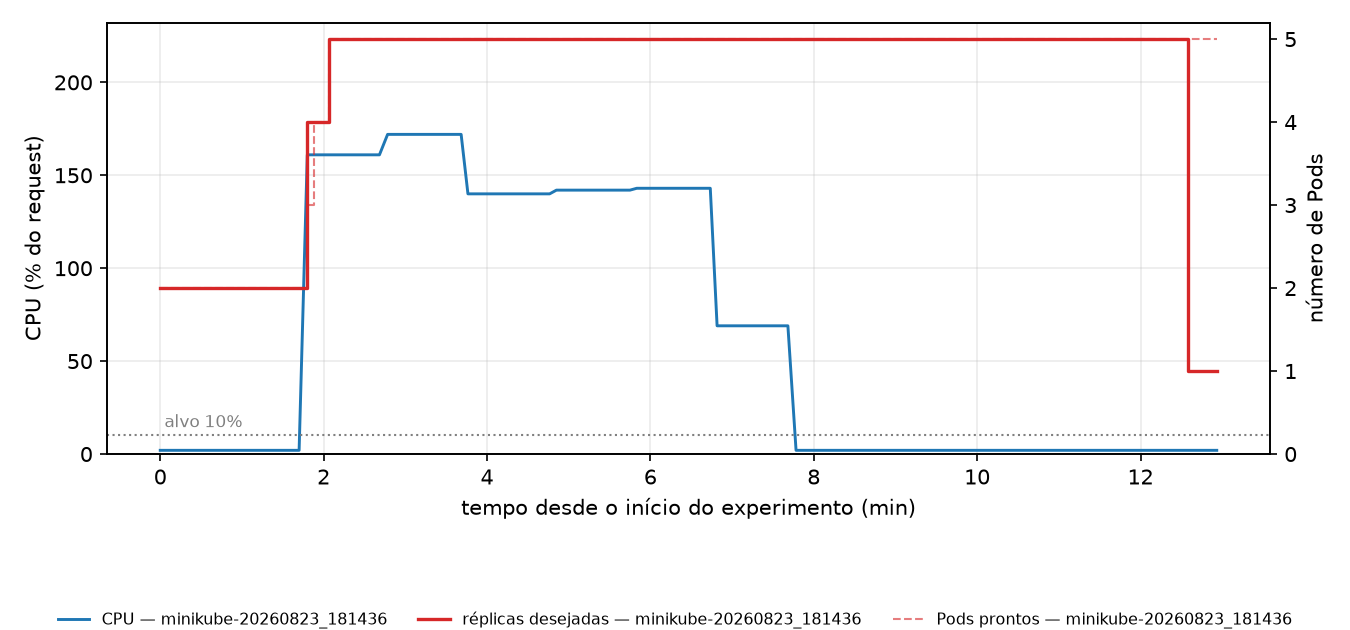
\includegraphics[width=\textwidth]{figuras/hpa-minikube.png}
\caption{Implantação A (Minikube): utilização de CPU e número de Pods ao
  longo das três fases do experimento. A linha pontilhada marca o alvo de
  10\% do \textit{request}.}
\label{fig:minikube}
\end{figure}

% Figura da Implantacao B - inserir quando o experimento no EKS terminar.
%\begin{figure}[ht]
%\centering
%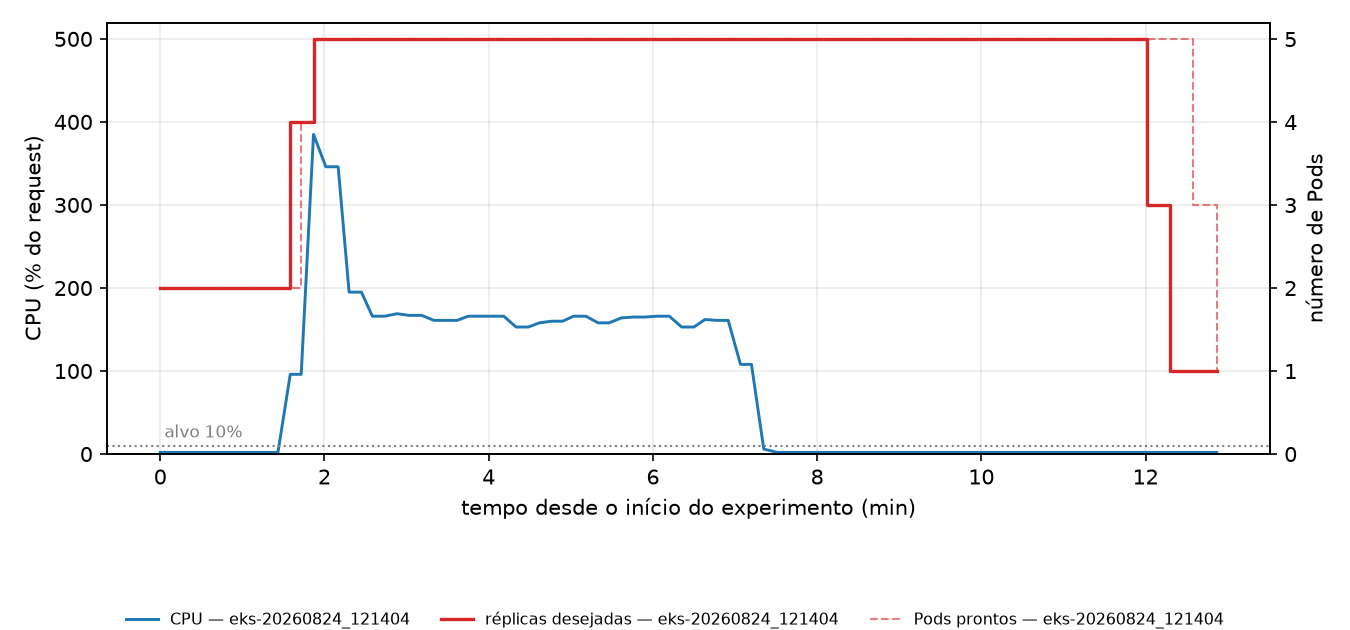
\includegraphics[width=\textwidth]{figuras/hpa-eks.png}
%\caption{Implantação B (Amazon EKS): mesma escala e mesmos parâmetros.}
%\label{fig:eks}
%\end{figure}

% =============================================================================
% SECAO 6 -- CONCLUSOES
% RESPONSAVEL: Franco (integracao)
% ALVO: 0,5 pagina
% =============================================================================
\section{Conclusões e considerações finais}

% O que precisa aparecer aqui:
%  - retomar o achado central: o ALGORITMO do HPA e o mesmo nos dois
%    ambientes; o que muda e o substrato, e o substrato aparece na defasagem
%    entre a decisao e a disponibilidade efetiva das replicas;
%  - a assimetria subir/descer como decisao de engenharia, nao defeito;
%  - a licao de custo: no EKS o desperdicio nao vem da carga, vem do tempo
%    ocioso - plano de controle e balanceador cobram por hora
%    independentemente de trafego;
%  - LIMITACOES, com honestidade: um unico node group sem autoescalamento de
%    nodes; servidor single-thread; alvo de 10% escolhido para tornar o efeito
%    visivel e nao representativo de producao; uma unica execucao por ambiente,
%    sem repeticoes nem intervalo de confianca;
%  - trabalhos futuros: HPA por metricas customizadas, Cluster Autoscaler ou
%    Karpenter, comparacao com Fargate e com EKS Auto Mode.

% =============================================================================
\bibliographystyle{sbc}
\bibliography{referencias}

\end{document}
